%%%%%%%%%%%%%%%%%%%%%%%%%%%%%%%%%%%%%%%%%%%%%%%%%%%%%%%%%%%%%%%%%%% 
%                                                                 %
%                           Resultaten                            %
%                                                                 %
%%%%%%%%%%%%%%%%%%%%%%%%%%%%%%%%%%%%%%%%%%%%%%%%%%%%%%%%%%%%%%%%%%% 
 
\chapter{Resultaten}\label{ch:resultaten}

\section{Object detectie}

Zoals besproken in hoofdstuk~\ref{sec:object_detectie} wordt er gebruik gemaakt van YOLOv2 met een aangepaste versie van darknet ge\"{i}mplementeerd in C.
Voor de training hebben we gebruik gemaakt van het standaard trainingsprogramma, voor het gebruik of inferentie van het netwerk maken we gebruik van
de Python api via de darknet 'shared library'.

De training en inferentie zijn beide gebeurd op een computer met de specificaties weergegeven in tabel~\ref{tab:specs}.

\begin{table}[!h]
    \caption{Computer specificaties}
    \label{tab:specs}
    \centering
    \begin{tabular}{l|l|l|l}
        & Model & Kloksnelheid & Geheugen \\
        \hline
        CPU & Ryzen 5 1600 & 4.0Ghz & 16 GB DDR4 \\
        GPU & GTX 1070 & 1.5Ghz & 8 GB GDDR5
    \end{tabular}
\end{table}

\subsection{Training}

We hebben 2 verschillende detectors getraind namelijk een detector op alle 4 de klassen (light, smoke\_detector, exit\_sign en door\_handle), en een detector
die enkel lampen kan detecteren.
Beide detectors zijn getraind op dezelfde dataset van 899 frames zoals reeds weergegeven in tabel~\ref{tab:annotaties}.
Voor de 2de detector hebben we de annotatie files aangepast zodat ze nog enkel lampen bevatten.
De detectors hebben beide een training gehad van 36000 iteraties met 64 afbeeldingen per iteratie.

\subsection{Snelheid}

De belangrijkste reden dat we voor de YOLOv2 detector gekozen hebben is de mogelijk om real-time te infereren.
Om dit aan te tonen is er een random sample van 100 frames genomen uit de datasets. Alle waarden zijn een gemiddelde van deze 100 afbeeldingen.

\begin{figure}
    \includegraphics[width=\linewidth]{results/yolo_420_lights.png}
    \caption{Inferentie van YOLOv2 detector met 1 klasse op 100 afbeeldingen.}
    \label{fig:speed_lights}
\end{figure}

In figuur~\ref{fig:speed_lights} hebben we dezelfde 100 afbeeldingen geinfereerd met de detector die enkel lampen detecteert.
Hierop kunnen we duidelijk afleiden dat de \gls{CPU} versie niet bruikbaar is voor real-time gebruik, maar de \gls{GPU} versie
met zijn $0.0271 s$ inferentie tijd of $36.9 fps$ zeker bruikbaar is. We zullen verder enkel de resultaten verkregen via \gls{GPU}
gebruiken omdat deze substantieel beter zijn.

\begin{figure}[h]
    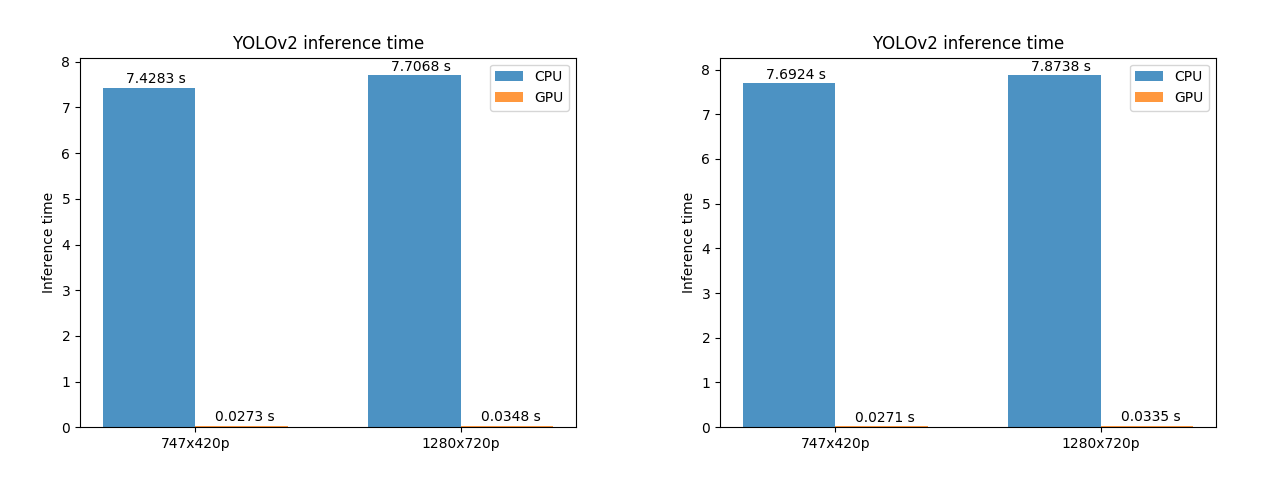
\includegraphics[width=\linewidth]{results/yolo_bar.png}
    \caption{Inferentie van YOLOv2 detector op verschillende inputformaten. \textbf{Links:} 4 klassen, \textbf{Rechts:} 1 klasse}
    \label{fig:speed_bar}
\end{figure}

Een belangrijke factor die invloed heeft op de inferentietijd is de grootte van de afbeeldingen die aan de detector als input gegeven worden
In figuur~\ref{fig:speed_bar} hebben we dezelfde input frames getest met een verschillende grootte, namelijk 1280x720 pixels en 747x420 pixels.
Zo kunnen we besluiten dat het verkleinen van de input frames met een factor 1.7 in de breedte en de hoogte een snelheidswinst kan opleveren van
ongeveer 20\%.

Een 2de conclusie die we kunnen opmaken uit figuur~\ref{fig:speed_bar} is dat het aantal detectieklassen slechts een kleine invloed heeft op de snelheid van de detector.


\subsection{Nauwkeurigheid}

Buiten de snelheid van de object detector is ook de nauwkeurigheid van belang.
Het testen van de nauwkeurigheid gebeurd door middel van een 2de dataset genaamd de validatieset. Deze validatieset bevat afbeeldingen genomen met dezelfde camera
van een ander deel van het gebouw, er zijn dus geen frames die de detector reeds gezien heeft tijdens de training.

De testprocedure begint door de detector te laten lopen op 1 frame, en de annotaties voor hetzelfde frame in te lezen.
Voor elke detectie wordt er gekeken of het label overeenkomt met het label in de annotatie.
Een 2de metriek waarmee rekening gehouden wordt is de Intersect Over Union(\gls{IoU}), zoals ge\"{i}llustreerd in figuur~\ref{fig:iou} is de \gls{IoU}
het oppervlak overeenkomstig tussen de detectie en de annotatie.
Een overlap van 100\% is perfect, een overlap van 0\% is slecht.

Uit deze 2 metrieken wordt de \gls{mAP} berekend, deze waarde geeft de oppervlakte onder de pr-curve.
De exacte berekeningen voor deze metrieken zijn beschreven in~\cite{everingham2010pascal}.

\begin{figure}[h]
    \centering
    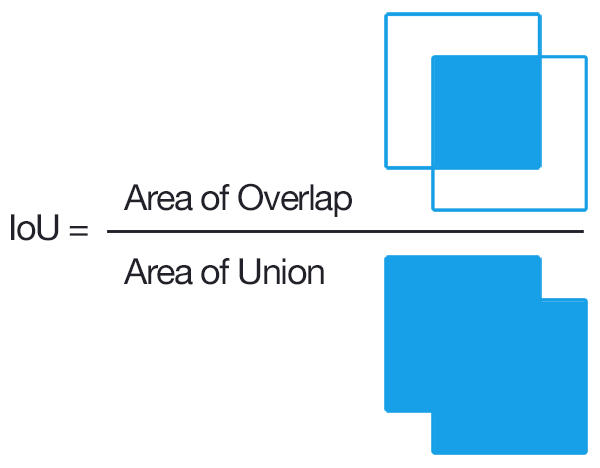
\includegraphics[width=0.5\linewidth]{results/iou.png}
    \caption{Grafische voorstelling IoU}
    \label{fig:iou}
\end{figure}

De pr-curves en \gls{mAP} waarden van onze detector zijn weergegeven in figuur~\ref{fig:yolo_pr}.

\begin{figure}[h]
    \includegraphics[width=\linewidth]{results/yolo_pr.png}
    \caption{Precision-Recall curves van YOLOv2 detector met mAP in de legende. \textbf{Links:} detector met 4 klassen. \textbf{Rechts:} detector met 1 klasse}
    \label{fig:yolo_pr}
\end{figure}

Uit de grafieken kunnen we een verband zien tussen de annotaties op het beeldmateriaal beschreven in tabel~\ref{tab:annotaties} en de nauwkeurigheid van
de detector voor bepaalde klassen. De klasse met het grootste aantal voorbeelden namelijk 'light' haalt de beste score.
De score voor 'door\_handle' of deurklink is nagenoeg 0, dit is niet verwonderlijk aangezien er slechts een paar voorbeelden waren in de dataset.
Dit object geeft dus geen meerwaarde voor de detector of voor het geheel.

Om deze reden is er getest of een detector met \'{e}\'{e}n enkele klasse betere resultaten zou opleveren.
De logische keuze voor de nieuwe klasse is uiteraard 'light' omdat deze de hoogste precisie haalt, maar ook het belangrijkste object is voor de lokalisatie.
In figuur~\ref{fig:yolo_pr} zien we echter dat dit weinig verschil maakt, de \gls{mAP} van de 2 detectors voor het lampobject is vergelijkbaar.

\section{Perspectiefpunt detectie}

In hoofdstuk~\ref{sec:perspectiefpunt_detectie} hebben is besproken hoe we drie verschillende methoden van perspectiefpunt detectie ge\"{i}mplementeerd hebben.
Hier gaan we de 3 technieken vergelijken op nauwkeurigheid en snelheid.


\subsection{Snelheid}\label{sec:seg_speed}
\begin{figure}[h]
    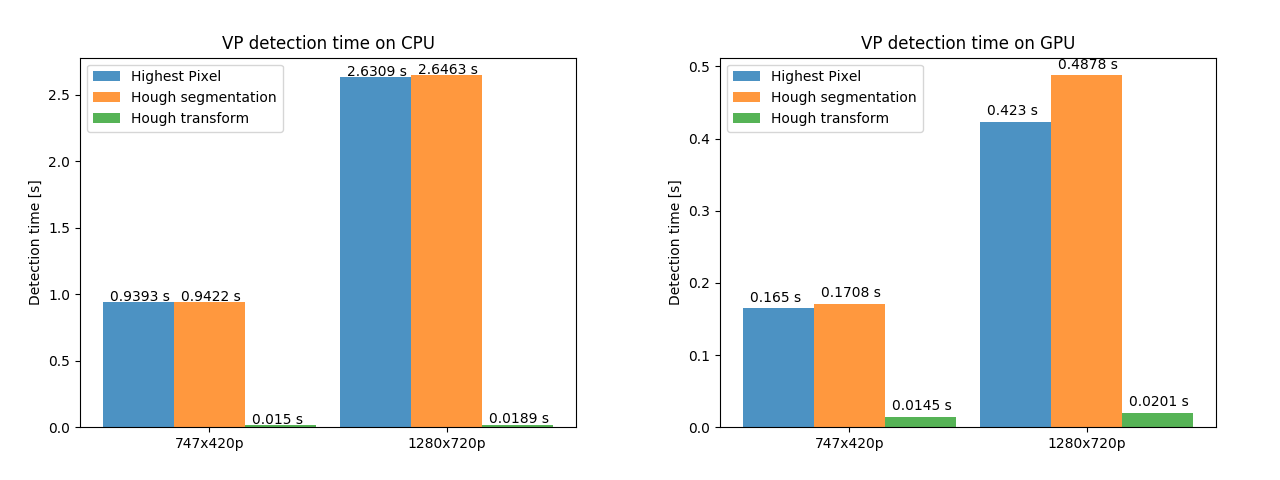
\includegraphics[width=\linewidth]{results/seg_speed.png}
    \caption{Detectiesnelheid van 3 perspectiefpunt detectiemethoden op CPU en GPU}
    \label{fig:seg_speed}
\end{figure}

In figuur~\ref{fig:seg_speed} zijn detectiesnelheden van de 3 detectietechnieken weergegeven.
Voor deze resultaten is het gemiddelde genomen van de detectietijd van 100 willekeurig gekozen input afbeeldingen uit de dataset.
Elke afbeelding is 4 keer door een specifieke detector gevalideerd namelijk op \gls{CPU} en \gls{GPU} alsook op 2 verschillende resoluties.
De verschillende resoluties zijn 1280x720 pixels en 747x420 pixels.

Net zoals bij de objectdetector zien we hier ook een aanzienlijk verschil in detectietijd tussen \gls{CPU} en \gls{GPU} voor 2 van de 3 technieken.
Dit is niet verwonderlijk aangezien deze methoden gebruik maken van een segmentatie netwerk.
Het verschil in tijd tussen \gls{CPU} en \gls{GPU} is zo groot dat we verder dus ook enkel de \gls{GPU} implementatie gaan gebruiken en bespreken.

Op de linkse grafiek in figuur~\ref{fig:seg_speed} is te zien dat de perspectieflijn kruising techniek met een grote marge de snelste techniek is, dit komt
omdat deze techniek gebaseerd is op klassieke beeldverwerkings technieken en geen gebruik maakt van een neuraal netwerk.
Hierbij is dan ook geen verschil tussen het detecteren op \gls{CPU} en \gls{GPU} omdat er geen \gls{GPU} implementatie is.

De hoogste vloerpixel techniek is de 2de snelste, deze techniek is een fractie sneller door zijn eenvoud na het segmenteren van de vloer.
Het zoeken van de hoogste pixel neemt amper tijd in beslag en het grootste deel van de tijd komt omwille van de segmentatie.

In figuur~\ref{fig:seg_speed} is ook duidelijk zichtbaar dat de resolutie van de input afbeelding een grote invloed heeft op de detectiesnelheid
van het gebruikte segmentatienetwerk.
Zo is door de afbeelding bijna te halveren in de breedte en de hoogte een snelheidswinst van ongeveer $60\%$ verkregen.


\subsection{Nauwkeurigheid}
Om de nauwkeurigheid van een perspectiefpunt detector te bepalen is er een script geschreven om voor elk van de 100 willekeurig gekozen input afbeeldingen
het perspectiefpunt handmatig aan te duiden.
Vervolgens is elke afbeelding getest door de 3 detectoren en het perspectiefpunt bepaald.
De co\"{o}rdinaten van het gedetecteerde perspectiefpunt, en het data punt door ons aangeduid, zijn beide in genormaliseerd ten opzichte van de breedte en de hoogte van de input afbeelding.
De euclidische afstand tussen de 2 punten is de afwijking of fout van de detector.

\begin{figure}[h]
    \centering
    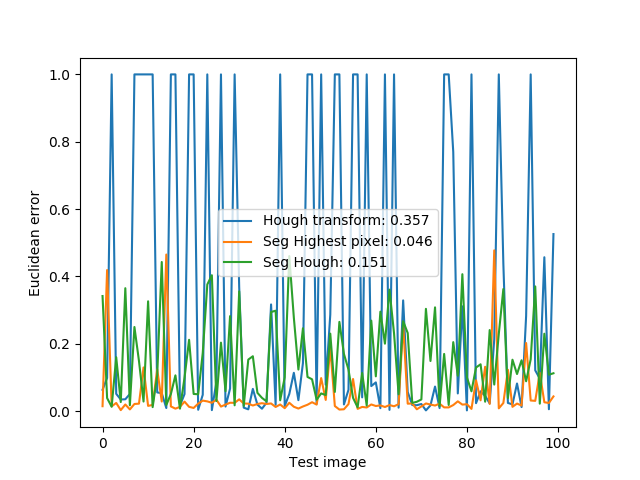
\includegraphics[width=0.6\linewidth]{results/seg_accuracy.png}
    \caption{Afwijking t.o.v. perspectiefpunt voor 3 verschillende detectietechnieken.}
    \label{fig:seg_accuracy}
\end{figure}

In figuur~\ref{fig:seg_accuracy} is de fout voor elke afbeelding weergegeven alsook de gemiddelde fout in de legende.
Hieruit kunnen we afleiden dat de perspectieflijn kruising techniek(\ref{sec:perspectieflijnkruising}) ondanks het de snelste techniek is, de laagste nauwkeurigheid haalt.
Dit is grotendeels omdat niet voor elke afbeelding de detector erin slaagt een perspectiefpunt te vinden. De reden dat niet in elk frame
een punt gevonden wordt komt door een gebrek aan hough-lines die gevonden worden op basis van de rand-detectie.
Door meer met de parameters te spelen zou dit probleem eventueel opgelost kunnen worden om de nauwkeurigheid van deze detector te verhogen.

Ondanks de eenvoudigste techniek te zijn, is de hoogste vloerpixel(\ref{sec:seg_highest}) methode over heel de lijn het meest nauwkeurig.
Een belangrijke reden voor dit resultaat is het excellente resultaat van het gebruikte segmentatienetwerk.
Indien de vloersegmentatie van mindere kwaliteit zou zijn, zou deze methode een slechter resultaat opleveren.

De vloerlijn kruising(\ref{sec:hough_floor}) methode geeft niet het beste resultaat, maar het is gemiddeld gezien zeker aanvaardbaar.
Doordat we in hoofdstuk~\ref{sec:seg_speed} besloten hebben dat de 2 technieken die gebruik maken van vloersegmentatie ongeveer evenveel rekentijd in beslag
nemen, en de hoogste vloerpixel methode de grootste nauwkeurigheid bied, is deze gekozen voor de uiteindelijke implementatie.


\section{Lokalisatie}

In de lokalisatiestap besproken in hoofdstuk~\ref{sec:lokalisatie} komt alles samen.
Hier zullen we bekijken hoe goed we een locatie kunnen inschatten op basis van semantische kenmerken in een \gls{rgb} beeld.
Zoals bij de vorige resultaten zijn ook deze opgesplitst in snelheid en nauwkeurigheid.


\subsection{Snelheid}
Voor validatie is er een dataset genomen van 125 opeenvolgende frames van een video.
De tijden waargenomen voor deze experimenten zijn voor 1 volledige iteratie in het programma, dit houd in:

\begin{itemize}
    \item YOLOv2 object detectie;
    \item Perspectiefpunt detectie;
    \item Lokalisatie berekeningen;
    \item User interface met frame en locatie op kaart plotten.
\end{itemize}

\begin{figure}[h]
    \centering
    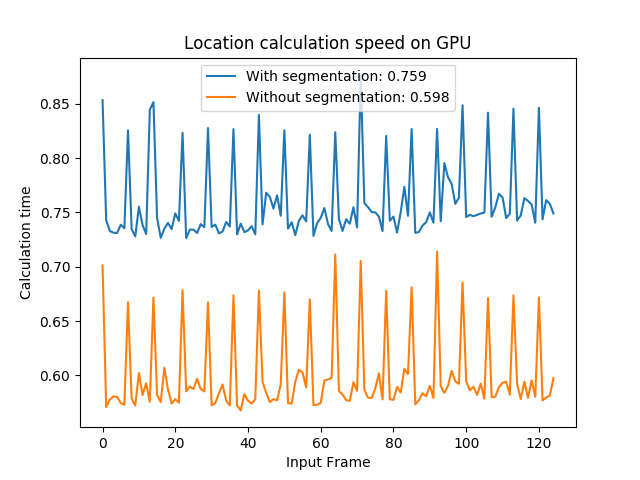
\includegraphics[width=0.6\linewidth]{results/loc_speed.png}
    \caption{Berekeningssnelheid van de actuele locatie}
    \label{fig:loc_speed}
\end{figure}

In figuur~\ref{fig:loc_speed} is een grafiek te zien van de iteratietijd per frame, in de legende is de gemiddelde tijd weergegeven.
Er is uiteraard een redelijk verschil waar te nemen tussen de implementatie die gebruikmaakt van het segmentatienetwerk, en die zonder.
Maar de detector zonder segmentatie(perspectiefpunt detectie d.m.v. perspectieflijn kruising~\ref{sec:perspectieflijnkruising}) heeft nog steeds
een vrij lange rekentijd.
Ondanks de theoretische snelheid die we uit vorige hoofdstukken kunnen afleiden ongeveer 0.042 s zou moeten zijn, is de gemiddelde rekentijd meer dan 10 keer hoger.
Na profilering van de implementatiecode, zijn we tot de constatatie gekomen dat het grootste deel van de tijd verloren gaat in de bibliotheek die gebruikt wordt
om de kaart en de actuele locatie visueel weer te geven. Dit is te zien in figuur~\ref{fig:loc_time}.
Hier zien we duidelijk dat de object en perspectiefpunt detector wel een stuk tijd in beslag nemen, maar dat door de visualisatie te laten vallen
de snelheid bijna $1/4$ van de huidige detectietijd zou kunnen zijn.

\begin{figure}[h]
    \centering
    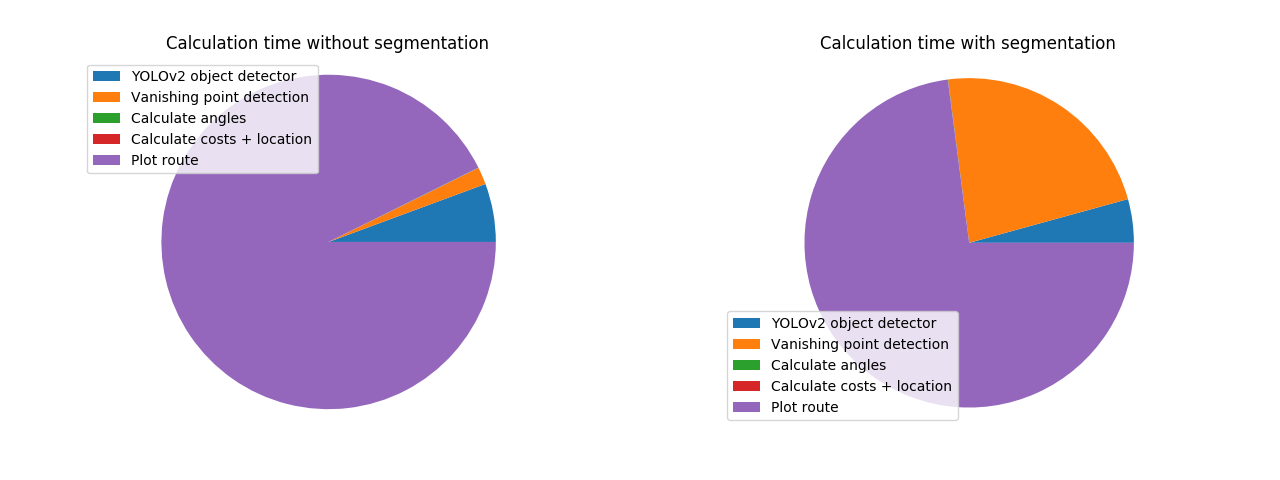
\includegraphics[width=\linewidth]{results/loc_time.png}
    \caption{Gemiddelde profilering van het lokalisatieproces}
    \label{fig:loc_time}
\end{figure}


\subsection{Nauwkeurigheid}
Voor de validatie is er op een dataset van 125 opeenvolgende frames van een video aangeduid bij welke discrete locatie op de semantische kaart
het beeld het beste past.
Deze data data wordt beschouwd als waarheid.
Dit wordt vergeleken met de output locatie per frame van ons programma.

\begin{figure}[h]
    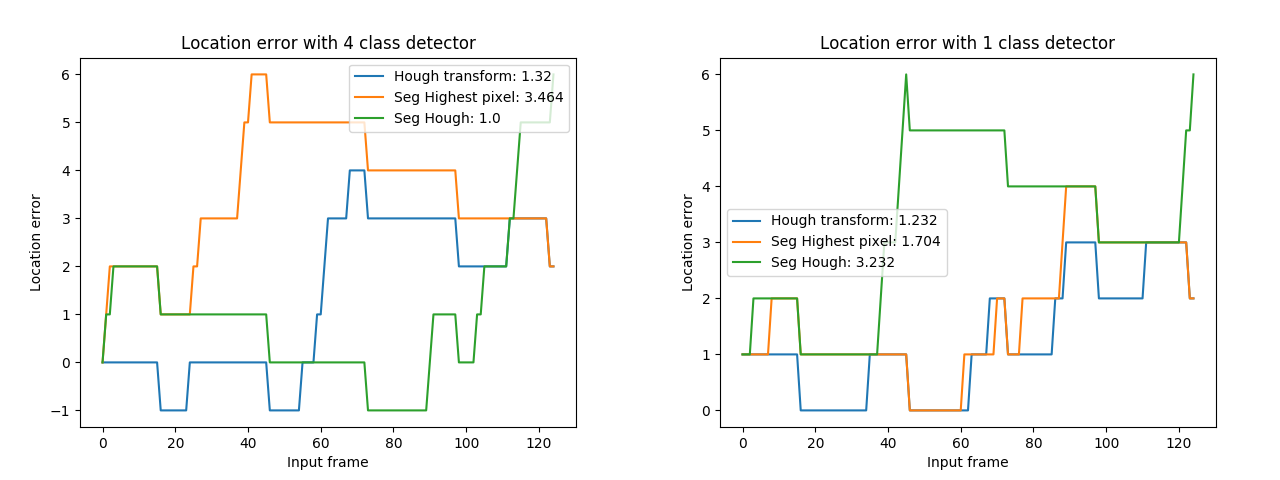
\includegraphics[width=\linewidth]{results/loc_acc.png}
    \caption{Vergelijking van lokalisatie fouten}
    \label{fig:loc_acc}
\end{figure}

In figuur~\ref{fig:loc_acc} is de fout in locatie weergegeven voor 6 verschillende detector combinaties.
Deze combinaties zijn de 2 YOLOv2 detectoren (4 klassen en 1 klasse) samen met de 3 perspectiefpunt detectiemethoden.

De locatiefout is het aantal nodes (beschreven in de route) dat de detector afwijkt van de actuele locatie.
Een fout van 0 is dus een juiste predictie, bij een positieve fout loopt de detector vooruit en bij een negatieve fout loopt de detector achter.
De legende in figuur~\ref{fig:loc_acc} geeft de gemiddelde fout van de geteste detector weer.

De grafieken geven duidelijk weer dat de lokalisatie niet altijd even goed verloopt.
Het algoritme heeft de neiging om te vaak vooruit te gaan, behalve bij 1 test is dit niet het geval waardoor de lokalisatie een beetje achterloopt.

De keuze van object detector kan een invloed hebben op de nauwkeurigheid. Dit komt omdat het aantal wel en niet gedetecteerde objecten
rechtstreeks gebruikt worden in scoreberekening~\ref{eq:score_weights}.
Een object met een grote wegingsfactor dat niet gedetecteerd is, zal zwaar afgestraft worden met een mogelijke lokalisatiefout ten gevolg.
Daarom zal het belangrijk zijn om een object detector te gebruikten met een grootte nauwkeurigheid.

Ook de keuze van perspectiefpunt detector heeft een grote invloed op de lokalisatie nauwkeurigheid.
Dit komt omdat de positie van het gedetecteerde punt rechtstreeks gebruikt wordt om de hoeken t.o.v. de gedetecteerde objecten te bepalen.
Als de hoeken niet nauwkeurig zijn, is het moeilijk om de metingen te linken aan een positie op de kaart.
Als in dit geval, door een slechte meting, de score van de verkeerde locatie hoger wordt, dan wordt er een verkeerde aanname gedaan.
Deze ene fout is misschien niet erg, maar wordt wel verder meegenomen in de volgende berekeningen waardoor de fouten zich kunnen opstapelen.

De belangrijkste reden voor de minder goede resultaten van de lokalisatie, is omdat de data in de semantische kaart niet nauwkeurig genoeg is.
Bij de start van het implementeren hebben we een semantische kaart verkregen met bijhorend beeldmateriaal van een specifieke omgeving.
Op dat moment bevatte de kaart enkel een beschrijving van de muren en deuren.
Dit was uiteraard niet genoeg voor de doeleinden die we hier voor ogen hadden, en was het noodzakelijk om de features beschreven in vorige hoofdstukken
in de kaart op te nemen.
Het was niet mogelijk om van deze objecten de echte afmetingen en locaties te verkrijgen, daarom is er besloten om op de kaart de afstanden en hoeken tot de objecten
te schatten. Deze schatting is gebeurd op basis van het verkregen beeldmateriaal.

Doordat onze data die slechts een schatting is, is het zeer moeilijk om exact te zeggen hoe nauwkeurig onze detector is.